% Unit circle
% Author: Supreme Aryal
% A unit circle with cosine and sine values for some
% common angles.
\documentclass[landscape]{standalone}
\usepackage{tikz}
\usepackage{fourier}
\usepackage[top=1in,bottom=1in,right=1in,left=1in]{geometry}
\begin{document}
    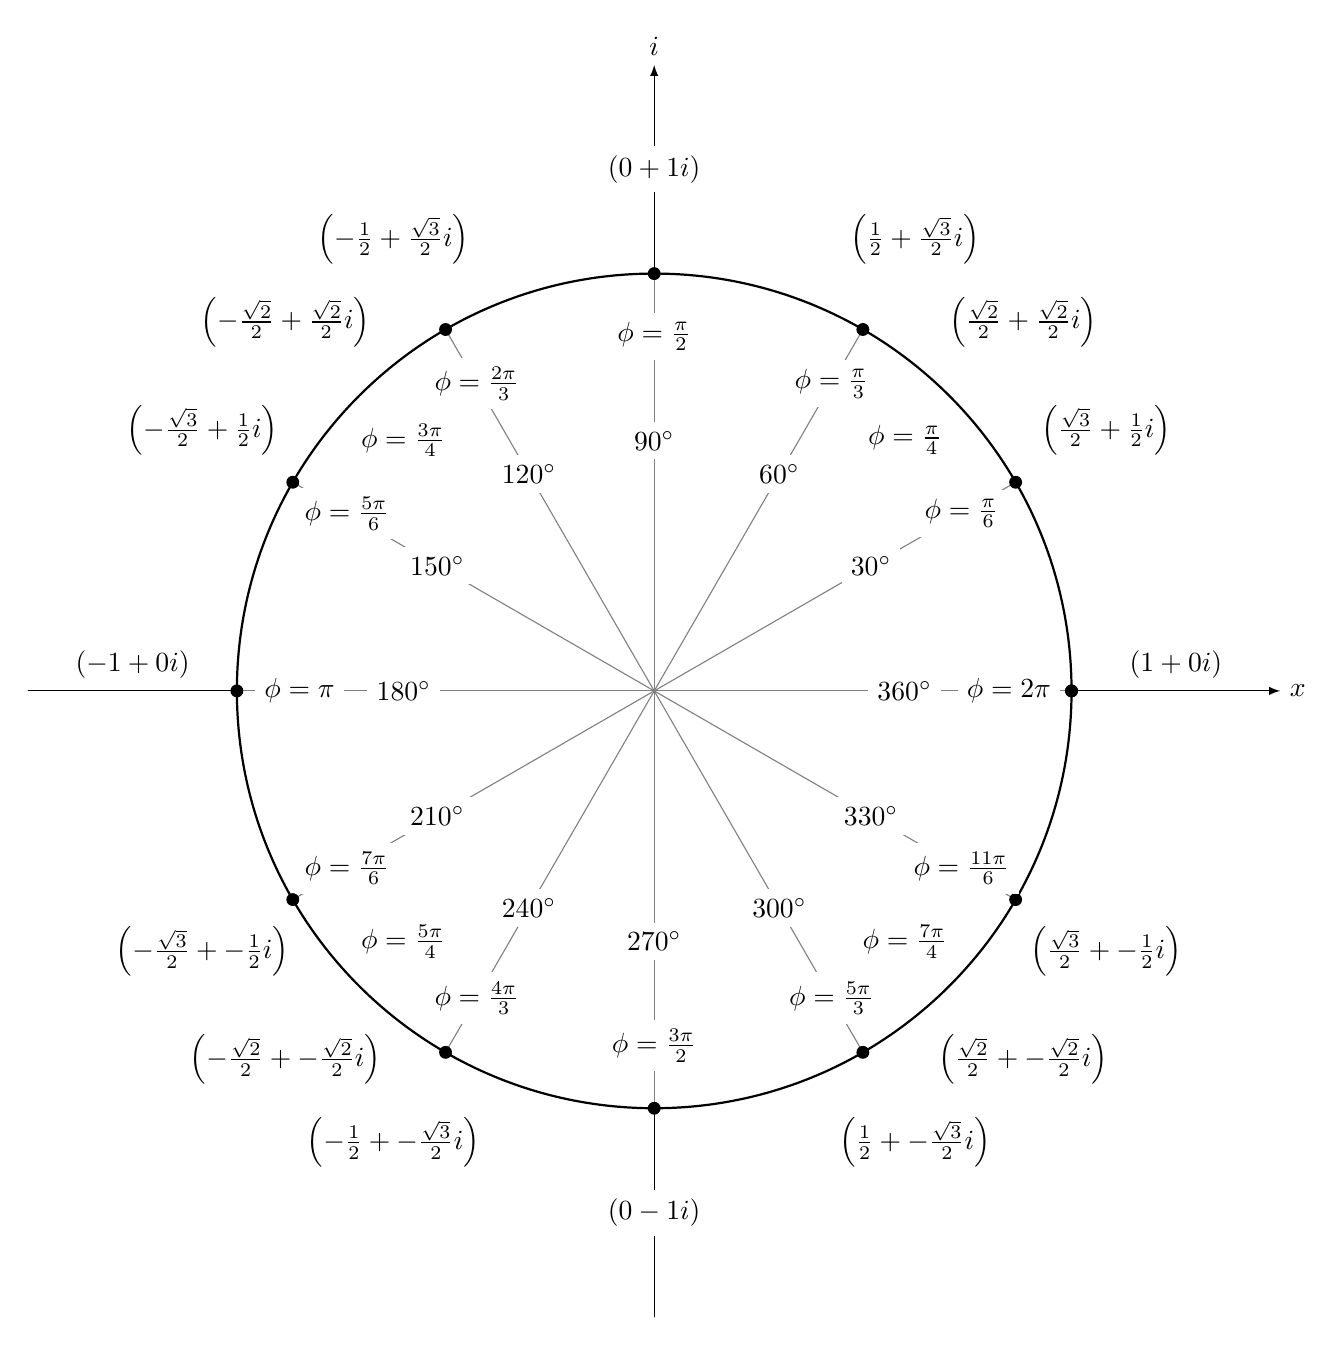
\begin{tikzpicture}[scale=5.3,cap=round,>=latex]
        % draw the coordinates
        \draw[->] (-1.5cm,0cm) -- (1.5cm,0cm) node[right,fill=white] {$x$};
        \draw[->] (0cm,-1.5cm) -- (0cm,1.5cm) node[above,fill=white] {$i$};

        % draw the unit circle
        \draw[thick] (0cm,0cm) circle(1cm);

        \foreach \x in {0,30,...,360} {
                % lines from center to point
                \draw[gray] (0cm,0cm) -- (\x:1cm);
                % dots at each point
                \filldraw[black] (\x:1cm) circle(0.4pt);
                % draw each angle in degrees
                \draw (\x:0.6cm) node[fill=white] {$\x^\circ$};
        }

        % draw each angle in radians
        \foreach \x/\xtext in {
            30/\phi = \frac{\pi}{6},
            45/\phi = \frac{\pi}{4},
            60/\phi = \frac{\pi}{3},
            90/\phi = \frac{\pi}{2},
            120/\phi = \frac{2\pi}{3},
            135/\phi = \frac{3\pi}{4},
            150/\phi = \frac{5\pi}{6},
            180/\phi = \pi,
            210/\phi = \frac{7\pi}{6},
            225/\phi = \frac{5\pi}{4},
            240/\phi = \frac{4\pi}{3},
            270/\phi = \frac{3\pi}{2},
            300/\phi = \frac{5\pi}{3},
            315/\phi = \frac{7\pi}{4},
            330/\phi = \frac{11\pi}{6},
            360/\phi = 2\pi}
                \draw (\x:0.85cm) node[fill=white] {$\xtext$};

        \foreach \x/\xtext/\y in {
            % the coordinates for the first quadrant
            30/\frac{\sqrt{3}}{2}/\frac{1}{2}i,
            45/\frac{\sqrt{2}}{2}/\frac{\sqrt{2}}{2}i,
            60/\frac{1}{2}/\frac{\sqrt{3}}{2}i,
            % the coordinates for the second quadrant
            150/-\frac{\sqrt{3}}{2}/\frac{1}{2}i,
            135/-\frac{\sqrt{2}}{2}/\frac{\sqrt{2}}{2}i,
            120/-\frac{1}{2}/\frac{\sqrt{3}}{2}i,
            % the coordinates for the third quadrant
            210/-\frac{\sqrt{3}}{2}/-\frac{1}{2}i,
            225/-\frac{\sqrt{2}}{2}/-\frac{\sqrt{2}}{2}i,
            240/-\frac{1}{2}/-\frac{\sqrt{3}}{2}i,
            % the coordinates for the fourth quadrant
            330/\frac{\sqrt{3}}{2}/-\frac{1}{2}i,
            315/\frac{\sqrt{2}}{2}/-\frac{\sqrt{2}}{2}i,
            300/\frac{1}{2}/-\frac{\sqrt{3}}{2}i}
                \draw (\x:1.25cm) node[fill=white] {$\left(\xtext + \y\right)$};

        % draw the horizontal and vertical coordinates
        % the placement is better this way
        \draw (-1.25cm,0cm) node[above=1pt] {$(-1+0i)$}
              (1.25cm,0cm)  node[above=1pt] {$(1+0i)$}
              (0cm,-1.25cm) node[fill=white] {$(0-1i)$}
              (0cm,1.25cm)  node[fill=white] {$(0+1i)$};
    \end{tikzpicture}
\end{document}
